\section{Document Clustering Techniques}

Scatter/Gather - first successful document clustering for information retrieval \cite{cutting1992scatter}


Types of clustering techniques:
\begin{itemize}
  \item hierarchical
  \item partitioning
  \item density-based
  \item etc
\end{itemize}


Cluster analysis: organizing collection of items into coherent groups

IR: need to assist user and group retrieved results into clusters 


Finding topics in a collection of document is an important task in text mining.
Usually done by applying a clustering technique and hope it will result 
if groups that represent documents in some common theme or topic \cite{ertoz2004finding}
The goal is to find clusters with strong coherent themes (even if we omit some documents)
in reality it's true: we don't expect all documents to belong to some strong category.

A group of documents with a strong topic is characterized by how it uses 
words from some specialized vocabulary in additional to general vocabulary. 

A doc about olympics would contain general terms (the, a) and specific terms (country names)


Data model \cite{ertoz2004finding} \ref{fig:topic-clusters}: there are concepts from which documents pick their words. DESCRIBE it.

\begin{figure}[h]
\centering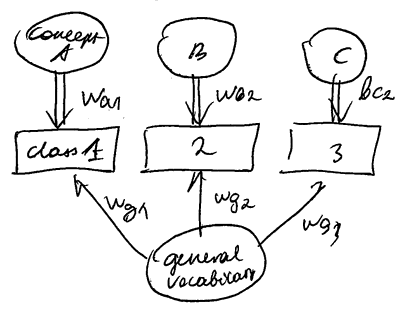
\includegraphics[width=0.5\textwidth]{data-model.png}
\caption{\textbf{TODO: }Abstract data model}
\label{fig:topic-clusters}
\end{figure}


\subsection{Hierarchical clustering}


 Agglomerative Clustering
General concept: merge items into clusters based on distance/similarity
usually based on best pairwise similarity

Typical steps:

- at the beginning each document is a cluster on its own
- then we compute similarity between all pairs of clusters and store the results in a similarity matrix
- merge two most similar clusters
- update the similarity matrix
- repeat until everything belongs to the same cluster


Linkage Types

How to join two clusters?
- Single Linkage (SLINK)
- Complete Linkage (CLINK)
- Group-Average Linkage
- Ward 



Single Linkage
Merge two groups $A$ and $B$ based on their closest pair


Implementation:
compute all similarity pairs
sort them in order of decrease
process pairs in this order


advantage:
efficient to implement
equivalent to a Spanning Tree algo on the complete graph of pair-wise distances can use Prim's Spanning Tree algo


Drawbacks
encourages chaining
similarity is usually not transitive:
i.e. if $A$ is similar to $B$, and $B$ is similar to $C$, it doesn't mean that $A$ must be similar to $C$
but single linkage encourages grouping through transitivity chains


References:
Sibson, Robin. "SLINK: an optimally efficient algorithm for the single-link cluster method." 1973. 


 Complete Linkage 
Worst-case similarity:
avoids chaining altogether
but it's very expensive computationally


References:
Defays, Daniel. "An efficient algorithm for a complete link method." 1977. 

Group-Average Linkage
similarity between groups $A$ and $B$ are calculated as average similarity between each $a \in A$ and $b \in B$


It's way slower than single linkage,
but it's more robust: it doesn't show the chaining behavior


Speeding up:
can approximate it by using the distance between centroids: mean doc in $A$ and mean doc in $B$



Ward's Method
Merge the pair of clusters that minimizes the total within-group error (sum of squares) between each document and centroid


Result:
spherical tightly bound clusters
less sensitive to outliers

References:
El-Hamdouchi, Abdelmoula, and Peter Willett. "Hierarchic document classification using Ward's clustering method." 1986. 


Pros and Cons
Single-link algorithms are best for capturing clusters of different sizes and shapes
but it's also sensitive to noise
complete link and group average are not affected by noise, but have a bias towards finding global patterns

Computational complexity:
only Single-Link is computationally possible for large datasets, but it doesn't give good results because uses too little information


\cite{steinbach2000comparison} - not always good for document clustering
because they make mistakes at early iterations that are impossible
to correct afterwards


\subsection{K-Means} \label{sec:kmeans}


Lloyd algorithm is the most popular way of implementing k-means


Algorithm 
 First we choose $k$ - the number of clusters we want to get
 Then we randomly initialize k cluster centers (cluster centroids)

This is an iterative algorithm, and on each iteration it does 2 things
 cluster assignment step
 move centroids step

Cluster Assignment Step:
 go through each example and choose the closest centroids
 and assign the example to it

Move Centroids Step:
 Calculate the average for each group
 and move the centroids there

Repeat this until converges


Pseudo Code

Let's have the following notation
$c_i \in \{ 1, 2, \ ... \ , k \}$ - index of cluster to which example $\mathbf x_i$ is assigned
$\boldsymbol \mu_k$ - cluster centroid $k$ ($\boldsymbol \mu_k \in \mathbb{R}^n$)
$\mu_{c_i}$ - cluster centroid of example $\mathbf x_i$

$k$-means($k$, $\{ \mathbf x_i, y_i \}$):

randomly initialize $k$ cluster centroids $\boldsymbol \mu = \Big( \mu_1, \mu_2, \, ... \, , \mu_k \Big) \in \mathbb{R}^{k + 1}$
repeat:
cluster assignment step:
for $i = 1$ to $m$:
$c_i \leftarrow$ closest to $\mathbf x_i$ centroid using [[Euclidean Distance]] $\text{dist} = \| \mathbf x_i - \boldsymbol \mu_i \|^2$
 move centroids step:
 for $i = 1$ to $k$:
 $\boldsymbol \mu_k \leftarrow$ average of all points assigned to $c_k$


Often K-Means shows the best results \cite{hall2012evaluating} \cite{steinbach2000comparison}, but it takes long for large collections.

Solution: minibatch K-means (web-scale k-means clustering paper) \cite{sculley2010web}

Lloyd's classical algorithm is slow for large datasets (Sculley2010)
Use [[Mini-Batch Gradient Descent]] for optimizing K-Means
reduces complexity while achieving better solution than [[Stochastic Gradient Descent]]

Notation:
$f(C, \mathbf x)$ returns the nearest centroid for $\mathbf x$


Algorithm:
 given $k$, batch size $b$, max. number of iterations $t$ and dataset $X$
 initialize each $\boldsymbol \mu$ with randomly selected elements from $X$
 repeat $t$ times:
 $M \leftarrow b$ random examples from $X$
 for $\mathbf x \in M$:
 $d[\mathbf x] = f(C, \mathbf x)$ // cache the centroid nearest to $\mathbf x$
 for $\mathbf x \in M$:
 $\boldsymbol \mu \leftarrow d[\mathbf x]$
 $v[\boldsymbol \mu] = v[\boldsymbol \mu] + 1$ // counts per centroid
 $\eta = 1 / v[\boldsymbol \mu]$ // per-centroid learning rate
 $\boldsymbol \mu \leftarrow (1 - \eta) \cdot \boldsymbol \mu + \eta \cdot \mathbf x$ //gradient step


If rows are unit-normalized, then Euclidean K-means is the same 
as Cosine Distance K-Means, but with convergence guarantees. 
TODO: ADD REFERENCE


\subsection{Extensions of K-Means} \label{sec:kmeans-ext}

Bisecting K-Means \cite{steinbach2000comparison}

This is a variant of K-Means
it's a [[Hierarchical Clustering]] method, and it's useful for [[Document Clustering]]


Algorithm:
start with a single cluster
 repeat until have desired number of clusters
 choose a cluster to split (e.g. the largest one)
 find two subclusters using K-means with $k = 2$ and split
 may repeat this procedure several times and take the clusters with highest overall similarity


Scatter/Gather \cite{cutting1992scatter}

This is
use [[Hierarchical Clustering]] for seed selection,
k-means for clustering

Scatter/Gather is a variation of [[K-Means]] used for [[Document Clustering]] with
special seed selection
usual k-means
then several cluster refinement operations


Idea:
use some hierarchical clustering algorithm on a sample to find good initial seeds
use K-Means afterwards

After selecting seeds just do usual K-Means
but do some additional operations to improve quality for document clustering


Cluster refinement hypothesis:
documents that belong to the same cluster in finer granularity will also occur in the same cluster in coarser granularity


Split Operations
The main idea is to continue splitting after K-Means has finished
sometimes clusters as not as granular as we'd like
continue splitting them to refine clusters
don't need to apply it to all clusters - only to non-coherent ones
it will help create more coherent clusters

(so it's just applying k-means once again on the cluster with $k=2$

Algo:
select a cluster to split
apply buckshot with $k=2$ on this cluster
re-cluster around these centers


How to measure "coherence"?
compute self-similarity of a cluster:
similarity of documents to the centroid cluster
or average pairwise similarity within the cluster
apply split only to clusters with low self-similarity


Join Operation
The idea:
after K-means has finished,
join very similar clusters into one


How?
compute typical words of each cluster:
i.e. examine most frequent words on the centroid
two clusters are similar if there's significant overlap between words of these clusters



Challenges
if there are many documents, the centroid will contain many word => leads to slowdown
solution: use [[Projection onto Subspaces|projection]] techniques like [[PCA]] 





Center adjustment (vector average dumping) \cite{larsen1999fast}

Smart seed selection \cite{cutting1992scatter} \cite{larsen1999fast}



\subsection{DBSCAN} \label{sec:dbscan}

describe the algo \cite{ester1996density}

It's a density-based clustering algorithm


Density associated with a point is obtained by counting the number of points in a region of specified radius $\epsilon$ around each point
 points with density $\geqslant \text{min\_pts}$ are considered as "core points"
 noise and non-core points are discarded
 clusters are formed around the core points
 if two core points are within a radius $\epsilon$, then they belong to the same cluster



Disadvantages
 can find clusters of different shapes, but can't find clusters of different densities

Pseudocode (taken from Wiki)

\begin{verbatim}
DBSCAN(D, eps, MinPts) {
   C = 0
   for each point P in dataset D {
      if P is visited
         continue next point
      mark P as visited
      NeighborPts = regionQuery(P, eps)
      if sizeof(NeighborPts) < MinPts
         mark P as NOISE
      else {
         C = next cluster
         expandCluster(P, NeighborPts, C, eps, MinPts)
      }
   }
}

expandCluster(P, NeighborPts, C, eps, MinPts) {
   add P to cluster C
   for each point P' in NeighborPts {
      if P' is not visited {
         mark P' as visited
         NeighborPts' = regionQuery(P', eps)
         if sizeof(NeighborPts') >= MinPts
            NeighborPts = NeighborPts joined with NeighborPts'
      }
      if P' is not yet member of any cluster
         add P' to cluster C
   }
}

regionQuery(P, eps)
   return all points within P's eps-neighborhood (including P)
\end{verbatim}

Can be adapted to take similarity measure instead of distance



\subsection{Extensions of DBSCAN} \label{sec:dbscan-ext}

SNN Clustering: \cite{ertoz2003finding}

Different similarity measure

Applicable to document clustering and discovering topics \cite{ertoz2004finding}

The goal:
find clusters of different shapes, sizes and densities in high-dimensional data
 [[DBSCAN]] is good for finding clusters of different shapes and sizes, but it fails to find clusters with different densities
it will find only one cluster:
 http://habrastorage.org/files/ff4/b40/6fc/ff4b406fc5d948d7bf3b2d4e3c18a71d.png
 (figure source: Ertoz2003)


Distance:
 [[Euclidean Distance]] is not good for high-dimensional data
 use different similarity measure in terms of [[KNN]]s - "Shared Nearest Neighbors"
 then define density in terms of this similarity


"Jarvis-Patrick" algorithm, as in Jarvis1973


Step 1: SNN sparsification:
 construct an SSN [[Graph]] from data matrix as follows
 if $p$ and $q$ have each others in the KNN list
 then create a link between them


Step 2: Weighting
 weight the links with $\text{sim}(p, q) = \big| \, \text{NN}(p) \ \cup \ \text{NN}(q) \, \big|$
 where $\text{NN(p)}$ and $\text{NN(q)}$ are $k$ neighbors of $p$ and $q$ resp.


Step 3: Filtering
 then filter the edges:
 remove all edges with weight less than some threshold


Step 4: Clusters
 let all connected components be clusters


Illustration
 http://habrastorage.org/files/b2b/174/cd8/b2b174cd84e3488a8d1dad51687bf194.png
 (figure source: Ertoz2003)
 note that this procedure removed the noise
 and clusters are of uniform density: it breaks the links in the transition regions


Usual density is not good:
 In the Euclidean space, the density is the number of points per unit volume
 but as dimensionality increases, the volume increases rapidly
 so unless the number of points increases exponentially with dimensionality, the density tends to 0
 Density-based algorithms (e.g. [[DBSCAN]]) will not work properly


Need different intuition of density
 can use a related concept from
 if $k$th nearest neighbor is close, then the region is most likely of high density
 so the distance to $k$th neighbor gives a measure of density of a point
 because of the [[Curse of Dimensionality]], the approach is not good for [[Euclidean Distance]], [[Cosine Similarity]] or others
 but we can use the SNN-Similarity to define density


SSN-based measures of density:
 sum of SSN similarities over all KNNs
 why sum an not just $k$th?
 to reduce random variation - which happens when we look only at one point
 to be consistent with the graph-based view of the problem
 of it can be the number of points within some radius - specified in terms of SNN distance
 like in [[DBSCAN]], but with SSN distance


SNN Clustering algorithm is a combination of
 Jarvis-Patrick algorithm and
 DBSCAN with SSN Similarity and SSN Density


Parameters
 $k$
 $\epsilon$
 $\text{min\_pts} < k$


Steps:
 compute the similarity matrix
 sparsify the matrix by keeping only $k$ most similar neighbors for each data point
 construct the SSN graph (use the Jarvis-Patrick algo)
 find SSN density of each point $p$:
 in the KNN list of $p$ count $q$ s.t. $\text{sim}(p, q) \geqslant \epsilon$
 find the core points
 all points with SSN density greater than $\text{min\_pts}$ are the core ones
 form clusters from the core points
 all non-core points not within $\epsilon$ from the core ones are discarded as noise
 align non-noise non-core points to clusters


Parameter tuning:
 $k$ controls granularity of clusters
 if $k$ is small, then it will find small and very tight clusters
 if $k$ is large, it'll find big and well-separated clusters


 The algorithm runs in $O(n^2)$ time
 can speed up with [[Kd-Trees]] or [[R-Tree]]s
 alternatively, can use [[Canopy Clustering|canopies]]


\subsection{Scaling?}

LSH etc
